\documentclass{article}
\usepackage[utf8]{inputenc} % Encodage pour les caractères spéciaux
\usepackage[T1]{fontenc}  
\usepackage{graphicx}
\usepackage[margin=1.8cm]{geometry}
\usepackage{fancyhdr}
\usepackage{pgf}
\usepackage{lmodern}
\usepackage{bold-extra}
\usepackage{pgfplots}
\usepackage{tikz}
\usepackage{todonotes}
\usepackage{setspace} 
\usepackage{titlesec}
\usepackage{gensymb}
\usepackage{amsmath,amsfonts,amssymb}
\usepackage[T1]{fontenc}
\usepackage{natbib} 
\usepackage[english]{babel}
\usepackage{hyperref}
\usepackage{lipsum}  
\usepackage{subcaption}
\usepackage{array}
\usepackage[table, dvipsnames]{xcolor}
\usepackage{textcomp}

\definecolor{darkblue}{rgb}{0.0, 0.0, 0.8}
\pgfplotsset{compat=1.9}
\usepgfplotslibrary{groupplots}
\usepgfplotslibrary{polar}
\usepgfplotslibrary{smithchart}
\usepgfplotslibrary{statistics}
\usepgfplotslibrary{dateplot}
\usepgfplotslibrary{ternary}
\setlength{\headheight}{12.80502pt}


\setcitestyle{authoryear,open={},close={}, color = 'blue'}

\hypersetup{colorlinks,linkcolor={blue},citecolor={blue},urlcolor={blue}}  

\DeclareCaptionFormat{custom}
{%
    \textbf{#1{.}} \small{#3}
}
\captionsetup{format=custom}

\renewcommand{\contentsname}{Contenu}

\titleformat{\section}
  {\Large\bfseries\scshape}{\thesection}{1em}{}
\titleformat{\subsection}
  {\large\scshape}{\thesubsection}{1em}{}
\titleformat{\subsubsection}
  {\scshape}{\thesubsubsection}{1em}{}

%\setlength{\arrayrulewidth}{1mm}
%\setlength{\tabcolsep}{9pt}
\renewcommand{\arraystretch}{1.5}
%\newcolumntype{s}{>{\columncolor[HTML]{AAACED}} p{3cm}}

\renewcommand{\abstractname}{\sc \large Résumé}

\fancypagestyle{main}{
  \fancyhf{}
  \fancyfoot[L, RO]{\thepage}
%  \fancyhead[LO]{\firstleftmark}
  \fancyhead[C]{\sc Étude de spectres infrarouges de géantes rouges évoluées}
}




\pagestyle{main}

\begin{document}


\begin{titlepage}

\begin{minipage}{.3\textwidth}%
        \centering
        
\includegraphics[width=1.\textwidth]{LOGO_Universite__libre_bruxelles.png}\par\vspace{0.2cm}
        \end{minipage}%
        \hfill
        \begin{minipage}{.25\textwidth}%
        \centering
        
\includegraphics[width=1.\textwidth]{sciences_logo}\par\vspace{0.2cm}
        \end{minipage}%

\centering	\vspace{4cm}
	{\large Mémoire présenté en vue de l'obtention du diplôme de Master en
Sciences Physiques}\par\vspace{0.8cm}
	\rule{0.5\linewidth}{1pt}
	\vspace{0.8cm}\par 
	{\huge \textsc{Étude de spectres infrarouges d'étoiles géantes rouges évoluées} \par}
	\vspace{0.8cm}
	\rule{0.5\linewidth}{1pt}
	\vspace{1cm} \par 
	{\Large \textsc{Département de physique}} \par 
	{\Large \textsc{Institut d'Astronomie et d'Astrophysique}}\par\vspace{0.8cm}\vspace{3cm} \par 
	réalisé par\par
        {\large Margaux \textsc{Vandererven}\par \vspace{1cm} \par         
        }
		supervisé par\par
	\large Sophie \textsc{Van Eck}
	\vfill

% Bottom of the page
	{\large Année académique 2024-2025 \par}

\end{titlepage}



\pagestyle{empty}
\vfill

\centering	
	{\LARGE \textsc{Étude de spectres infrarouges d'étoiles géantes rouges évoluées} \par}
	\vspace{0.5cm}
	{\textsc{Institut d'Astronomie et d'Astrophysique}}\par\vspace{0.1cm} \par 
	\rule{0.3\linewidth}{0.4pt} \par
	\vspace{0.5cm}
	Margaux \textsc{Vandererven}\par \vspace{0.7cm} \par 
	\vspace{0.cm}
	
	
\abstract{\noindent La poussière}

\vspace{0.9cm}

\tableofcontents

\clearpage

% \pagestyle{main}
\section{\sc Introduction}

\section{\sc Débroussailler}


\section{\sc Molécules}

Synthèse avec modèle : 

\begin{table}[h!]
  \begin{center}
  \begin{tabular}{ccccccc}
      \hline
      \hline
      Modèle & $T_{\rm eff}$ (K) & log $g$ (cm $s^{-2}$) & [Fe/H] (dex) & Mass (M$_\odot$) & [s/Fe] (dex)\\
      \hline
      A &  $4000$ & $1.00$ & -0.50 & 1.0& +0.00 \\
      \hline
  \end{tabular}
  \end{center}
  \textbf{Notes.} 4000g1.0z-0.50m1.0t02a+0.20c+0.346n+0.00o+0.20r+0.00s+0.00
  \caption{Modèles de MARCS utilisés pour les synthèses.}
  \label{MARCS}
  \end{table} 
TODO: parler des modèles MARCS et de la grille de modèles.

Les listes de raies nous ont été fournies par Thomas Masseron, la provenance détaillée est donnée en Table \ref{origine_mol}. \par

 \begin{table}[h!]
  \vspace{0.3cm}
 \begin{center}
	\begin{tabular}{cc}
        \hline
		\hline
        Molécules & Auteur \\
        \hline
        $^{16}$OH & Brooke \\
        $^{56}$FeH & Dulick + Hargreaves \\
        $^{28}$SiO & Barton exomol \\
        $^{28}$SiH & Yurchenko2017(EXOMOL) \\
        HCl & HITRAN \\
        $^{12}$CH & Masseron2014 \\
        $^{13}$CH & Masseron2014 \\
        AlH & Yurchenko 2018(EXOMOL) \\
        $^{12}$C$^{14}$N & Sneden web \\
        $^{13}$C$^{14}$N & Sneden web \\
        YO & HITRAN \\
        HF & PGopher \\
        $^{12}$C$^{16}$O & HITRAN (Li 2018) \\
        $^{13}$C$^{17}$O & HITRAN (Li 2018) \\
        $^{48}$TiO & toto Exomol \\
        H$^{12}$CN & Exomol \\
        H$^{13}$CN & Exomol \\
        $^{52}$CrH & Burrows 2002 \\
        ZrO & toto Exomol \\
        $^{13}$C$^{13}$C & EXOMOL\\
        $^{12}$C$^{13}$C & EXOMOL\\
        $^{12}$C$^{12}$C & EXOMOL\\
        MgH & Yadin (EXOMOL) \\
        C$_2$H$_2$ & HITRAN \\
        VO & VOMYT \\
        $^{14}$NH &  Brooke edited by EXOMOL \\
        H$_2$O & Barber \& Tennyson \\
        $^{20}$CaH & Yadin (EXOMOL) \\
    \end{tabular}
\end{center} 
\caption{Provenance détaillée des listes de raies moléculaires.}
\label{origine_mol}
\textbf{Notes.}
\end{table}

 Les listes de raies atomiques ont la forme suivante :  \newline

 Je m'appelle margaux 

 longeur d'onde (Å) -\ excitation (eV) -\ log gf -\ log gf -\ fdamp -\ gup \newline
%  - gamma_rad - gamma_stark - s,p,d,f (upper level) - s,p,d,f (lower level) - largeur eqwuidt - error sur eqw - text - lower level number in NLTE model -  same for upper  - lower level id - upper level id" (cf. docs de turbospectrum)" \\ 

% ... in the fourth column of the line list (called fdamp):
% * 1) use ABO theory (Anstee, Barklem, O'Mara) for collisional damping with H,
% *    with data taken from line list: fdamp contains sigma.alpha.
% *    This number is available starting with VALD3 version of the VALD database.
% *    See : http://www.astro.uu.se/~barklem/howto.html
% * 2) if (1) not available check if something can be computed in the anstee.f
% *    routine using generic broadening recipes from the ABO formalism
% * 3) if (2) not available, check in linelist for a gamma6 at 10000K
% * 4) if nothing else worked, compute Unsoeld approximation, using a fudge factor
% *    read from column 4.


\begin{table}[h!]
%\caption{Listes de molécules et contribution de chacune d'elle dans la bande H et K}
\vspace{0.3cm}
\begin{minipage}[t]{.4\linewidth}
\begin{center}
	\begin{tabular}{cccc}
        \hline
		\hline
        Molécules & Bande H & Bande K & Cat. \\
        \hline
        $^{12}$C$^{14}$N & 55.14 \% & 44.35 \% & I\\
        $^{13}$C$^{14}$N & 32.00 \%  & 14.51 \%& I \\
        $^{12}$C$^{16}$O & 75.33 \% & 72.01 \% & I\\
        $^{13}$C$^{17}$O & 0.04 \% & 1.96 \% & II\\
        $^{16}$OH & 59.68 \% & 31.59 \% & I\\
        $^{56}$FeH& 3.12 \% & 0.08 \% & II\\
        HF & 17.79 \%  & 57.16 \%  & I\\
        $^{12}$CH & 4.68 \% & 10.68 \% & I\\
        $^{13}$CH & 0.15 \% & 0.39 \% & III\\
        $^{14}$NH & 1.57 \% & 1.23 \% & II\\
        $^{12}$C$^{12}$C & 32.97 \% & 30.73 \%& I \\
        $^{12}$C$^{13}$C & 14.12 \% & 12.26 \% & I\\
        $^{13}$C$^{13}$C & 0.38 \% & 0.25 \% & III\\
        C$_2$H$_2$ &  0.00  \% & 0.00 \% & III\\
        HCl & 0.64 \% &  0.50 \% & III\\
		H$_2$O & 1.75 \% & 6.80 \% & II\\
        $^{20}$CaH & < 0.01  \% & < 0.01  \% & III\\
        \hline
    \end{tabular}
\end{center} 
\end{minipage} 
\hspace{2.cm}
\begin{minipage}[t]{.4\linewidth}
\begin{center}
   \begin{tabular}{cccc}
        \hline
		\hline
        Molécules & Bande H & Bande K & Cat. \\
        \hline
        $^{28}$SiH & < 0.01 \% & 0.02 \% & III\\
        $^{28}$SiO & < 0.01 \% & 0.04 \% & III\\
		VO &  0.03 \% &  < 0.01 \% & III\\
		YO & < 0.01 \% &  < 0.01 \%& III\\
		$^{48}$TiO &  0.06 \% &  < 0.01 \% & III\\
		$^{24}$MgH &  < 0.01 \% &  < 0.01 \% & III \\
		AlH &  < 0.01 \% &  < 0.01 \% & III \\
		$^{52}$CrH & < 0.01 \% & 0.00 \% & III\\
		H$^{12}$CN & < 0.01 \% & < 0.01 \% & III\\
		H$^{13}$CN &   < 0.01 \% & < 0.01 \% & III\\
		$^{90}$ZrO & 0.02  \% & < 0.01  \% & III\\
		$^{91}$ZrO &  < 0.01 \% &  < 0.01 \% & III\\
		$^{92}$ZrO & < 0.01 \% &  < 0.01 \% & III\\
		$^{93}$ZrO &  0.00 \% & 0.00 \% & III\\
		$^{94}$ZrO &  < 0.01 \% &  < 0.01 \% & III\\
		$^{96}$ZrO &  < 0.01 \% &  < 0.01 \% & III\\
		 &  &  \\
        \hline
    \end{tabular}
	\end{center}
\end{minipage}
\vspace{0.3cm}

\textbf{Notes.} La catégorie I concerne les molécules contribuant à plus de 10\%, la catégorie II celles à moins de 10\% et plus de 1\% et la catégorie III celles à moins de 1\%. Les valeurs dans le colonne "Bande H" et "Bande K" sont le pourcentage en absorption du plus grand extremum du tracé de la différence entre le spectre synthétique atom + mol et le spectre synthétique atomique simple. log$\epsilon_C$ = 9,44, log$\epsilon_O$ = 9,56 et log$\epsilon_N$ = 8,38, MACturb = 8,00 kms-2, MICROturb = 1,70 et z = -0,3, ratio C = , ratio C/O=0.75.
\label{contribution_mol}
\end{table}

on garde du coup 3 listes de raies atomiques et 14 listes de raies moléculaires.

\section{\sc TS}

\section{\sc Minimisation \texorpdfstring{$\chi^2$}{chi-squared}}

$$\chi^2 = \sum \frac{(\text{synth\'etique}-\text{observ\'e})}{\text{observ\'e}}$$

on fait passer une fonction quadratique sur les valeurs de chi2 et on regarde le minimum.
si deux valeurs, on interpole une grille et on regarde le minimum.
TODO: mettre plot pour expliquer la minimisation. 

\section{Macroturbulence}
Nous commençons par déterminer la macroturbulence à l'aide de raies propres dans le bande H et K. Nous effectuons des synthèses avec le modèle A de la Table~\ref{MARCS} et les abondances CNO et paramètres stellaires de la littérature \cite{shetye_s_2018}. Nous procédons par minimisation $\chi^2$ sur différentes raies propres avec comme paramètre libre l'abondance de l'élément et la macroturubulence. 
Les autres abondances sont scale à partir de \cite{grevesse_solar_2007}.

\begin{table}[h!]
%\caption{Listes de molécules et contribution de chacune d'elle dans la bande H et K}
\vspace{0.3cm}

\begin{center}
	\begin{tabular}{ccccccc}
        \hline
		\hline
        Élément & $\lambda$ (Å) & $\lambda_{\mathrm{min}}$ (Å) & $\lambda_{\mathrm{max}}$ (Å)& v$_{\mathrm{macro}}$ ($km s^{-1}$) & log $\varepsilon$ & $\chi^2$\\
        \hline
    Fe I & 15964.865 &&& 8.58 && \\
    % raie de bande H
    Fe I & 22257.107 &22256.48&22257.87& 8.65 &7.10& 0.0270\\
    Fe I & 22260.18 &22259.67&22260.77& 8.64 & 7.09 & 0.0132\\
		Co I & 16757.704&& & 8.61 && \\
		Ti I & 22211.22 & 22210.52 & 22211.91 & 8.90 & 4.88 & 0.0004\\
		Ti I & 22232.844&& & 9.00 &&\\
    \end{tabular}
\end{center} 
\textbf{Notes.} 
\label{macro}
\end{table}

\section{\sc Abondance CNO}
il n'y a pas de raies atomiques de C, N, O dans l'infrarouge, donc nous regarderons les molécules de OH pour l'abondance d'oxygène, de CO pour l'abondance de carbone et de CN pour l'abondance de carbone. 

Nous partons des paramètres stellaires de la littérature. [C/Fe]=0.35, [N/Fe]=-0.1, C/O=0.75
 log(C/O) = log$\epsilon_C$-log$\epsilon_O$

si on prend abu solaire de Magg 2022, 
[X/Fe] = log$\epsilon_*$ - log$\epsilon_{sun}$ - [Fe/H]
log$\epsilon_*$ = [X/Fe] + log$\epsilon_{sun}$ + [Fe/H]
= -0.1 + 7.98 -0.3 = 7.58 pour azote
log$\epsilon_{sun_N}$ = 7.98
log$\epsilon_{sun_O}$ = 8.77
log$\epsilon_{sun_C}$ = 8.56
log$\epsilon_*$ pour C = 0.35 + 8.56 - 0.3

Abondance d'oxygène avec raie de OH, Cabu=8.44 (litt) et Nabu=7.38 (litt) \cite{grevesse_solar_2007}
avec un ratio de 12C/13C à 40 (valeur standard pour géantes)
Données d'entrée :
0.35 +8.39 - 0.3 = 8.44 pour C
-0.1 +7.78 - 0.3 = 7.38 pour N
Paramètres variables : 
Oabu
macro 8.6 

% \begin{minipage}
%   \begin{figure}
%     \begin{center}
%       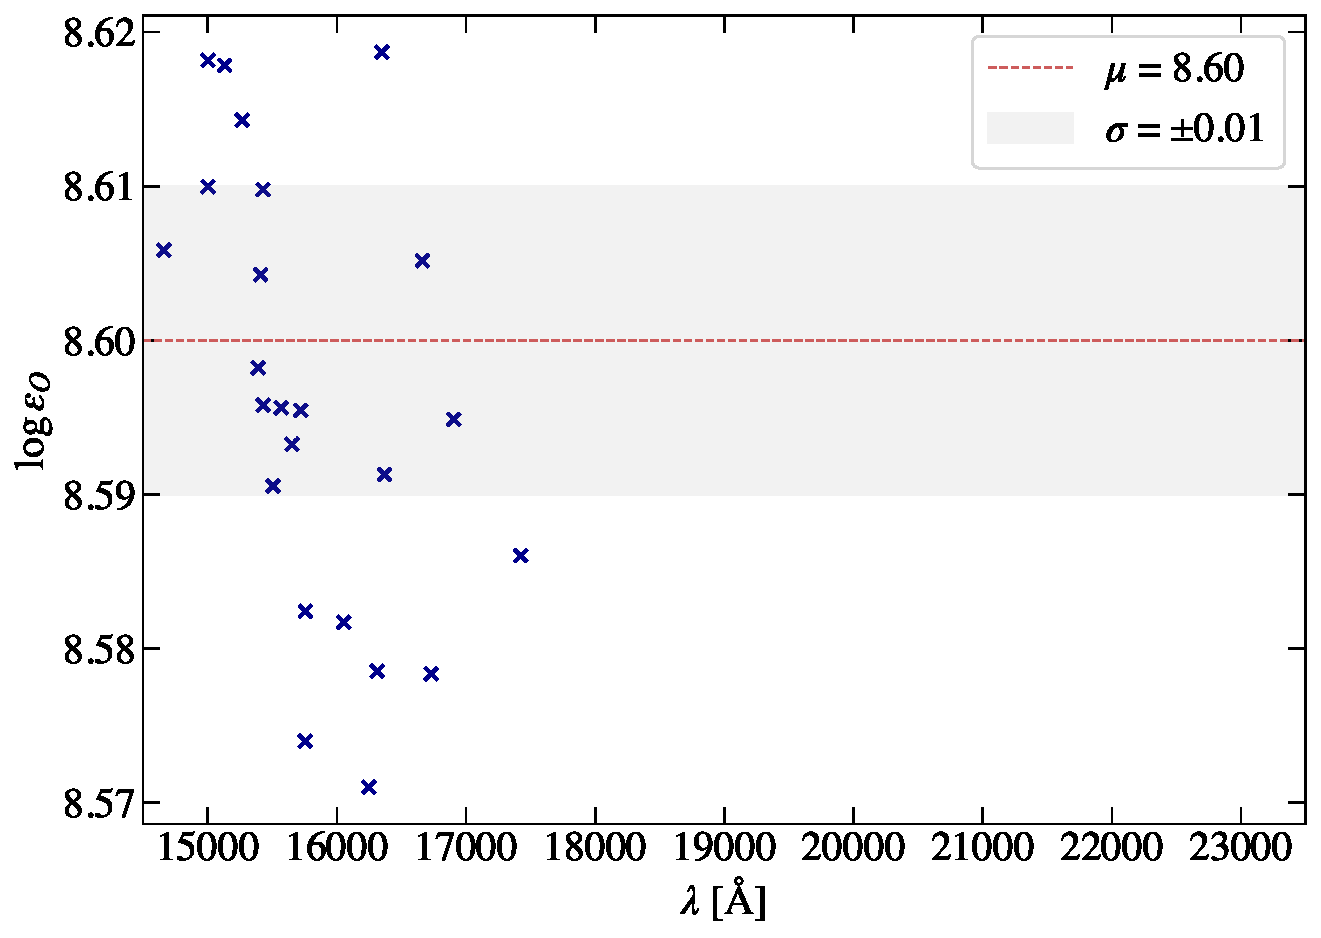
\includegraphics[width=10cm]{images/plot_abu/O_abu_first.pdf}
%     \end{center} 
%     \textbf{Notes.}  Abondance de O en fonction de la longueur d'onde pour la première itération. Abondance de C et N fixée à partir de la littérature. v$_{macro}$ 8.6 $km s^{-1}$. v$_{micro}$ 1.7 $km s^{-1}$. Modèle A de \ref{MARCS}
%   \end{figure}
% \end{minipage}
% \begin{minipage}
%   J'aimerais écrir ici 
% \end{minipage}


-> Oabu = 8.60 $\pm$ 0.01 voir Table \ref{itération_CNO}. 


Puis on repasse sur les raies de CO pour checker C avec donc Oabu = 8.59 et Nabu = 7.38 (litt)
tjrs ratio 12C/13C. 


\begin{table}[h!]
  \vspace{0.3cm}
\begin{center}
	\begin{tabular}{ccccc}
        \hline
		\hline
        log $\varepsilon_{\rm O}$ & log $\varepsilon_{\rm C}$ & log $\varepsilon_{\rm N}$ & $^{12}$C/$^{13}$C & Element\\
        \hline
    \textcolor{darkblue}{8.60 $\pm$ 0.01} & 8.44 & 7.38 & 40 & $^{16}$OH \\
    8.60 & \textcolor{darkblue}{7.79 $\pm$ 0.03} & 7.38 & 40 & $^{12}$C$^{16}$O \\
    8.59 & 7.82 & 7.38 & \textcolor{darkblue}{20} & $^{13}$C$^{17}$O \\
    \textcolor{darkblue}{8.30 $\pm$ 0.02} & 7.82 & 7.38 & 20 & $^{16}$OH \\
    8.30 & \textcolor{darkblue}{7.89 $\pm$ 0.02} & 7.38 & 20 & $^{12}$C$^{16}$O \\
    \textcolor{darkblue}{8.33 $\pm$ 0.02} & 7.89 & 7.38 & 20 & $^{16}$OH \\
    8.33 & \textcolor{darkblue}{7.86 $\pm$ 0.03} & 7.38 & 20 & $^{12}$C$^{16}$O \\
    8.33 & 7.86 & \textcolor{darkblue}{7.84 $\pm$ 0.02} & 20 & $^{12}$C$^{14}$N \\
    8.33 & 7.86 & 7.84 & \textcolor{blue}{12} & $^{13}$C$^{14}$N \\
    \textcolor{darkblue}{8.31 $\pm$ 0.01} & 7.86 & 7.84 & 12 & $^{16}$OH \\
    8.31 & \textcolor{darkblue}{7.88 $\pm$ 0.03} & 7.84 & 12 & $^{12}$C$^{16}$O \\
    8.31 & 7.88 & \textcolor{darkblue}{7.84 $\pm$ 0.02} & 12 & $^{12}$C$^{14}$N \\
    \end{tabular}
\end{center} 
\textbf{Notes.} 
Chaque synthèse est réalisée sur des raies de l'élement se trouvant en 4ème colonne. 
Les paramètres fixés sont en noir et le paramètre déterminé en bleu. 
\label{itération_CNO}
\end{table}

% \begin{table}[h!]
%   \vspace{0.3cm}
% \begin{center}
% 	\begin{tabular}{ccccc}
%         \hline
% 		\hline
%         log $\varepsilon_{\rm O}$ & log $\varepsilon_{\rm C}$ & log $\varepsilon_{\rm N}$ & $^{12}$C/$^{13}$C & Element\\
%         \hline
%     \textcolor{darkblue}{8.59 $\pm$ 0.01} & 8.44 & 7.38 & 40 & $^{16}$OH \\
%     % raie de bande H
%     8.59 & \textcolor{darkblue}{7.82 $\pm$ 0.03} & 7.38 & 40 & $^{12}$C$^{16}$O \\
%     8.59 & 7.82 & 7.38 & \textcolor{darkblue}{20} & $^{13}$C$^{17}$O \\
%     \textcolor{darkblue}{8.30 $\pm$ 0.02} & 7.82 & 7.38 & 20 & $^{16}$OH \\
%     8.30 & \textcolor{darkblue}{7.89 $\pm$ 0.02} & 7.38 & 20 & $^{12}$C$^{16}$O \\
%     \textcolor{darkblue}{8.33 $\pm$ 0.02} & 7.89 & 7.38 & 20 & $^{16}$OH \\
%     8.33 & \textcolor{darkblue}{7.86 $\pm$ 0.03} & 7.38 & 20 & $^{12}$C$^{16}$O \\
%     8.33 & 7.86 & \textcolor{darkblue}{7.84 $\pm$ 0.02} & 20 & $^{12}$C$^{14}$N \\
%     8.33 & 7.86 & 7.84 & \textcolor{blue}{12} & $^{13}$C$^{14}$N \\
%     \textcolor{darkblue}{8.31 $\pm$ 0.01} & 7.86 & 7.84 & 12 & $^{16}$OH \\
%     8.31 & \textcolor{darkblue}{7.88 $\pm$ 0.03} & 7.84 & 12 & $^{12}$C$^{16}$O \\
%     8.31 & 7.88 & \textcolor{darkblue}{7.84 $\pm$ 0.02} & 12 & $^{12}$C$^{14}$N \\
%     \end{tabular}
% \end{center} 
% \textbf{Notes.} 
% Chaque synthèse est réalisée sur des raies de l'élement se trouvant en 4ème colonne. 
% Les paramètres fixés sont en noir et le paramètre déterminé en bleu. 
% \label{itération_CNO_ancien}
% \end{table}

\newpage
\begin{figure}[htbp]
  \centering
  
  % Première image (graphique 1)
  \begin{subfigure}[b]{0.49\textwidth}  % Augmenter la largeur à 0.48\textwidth
      \centering
      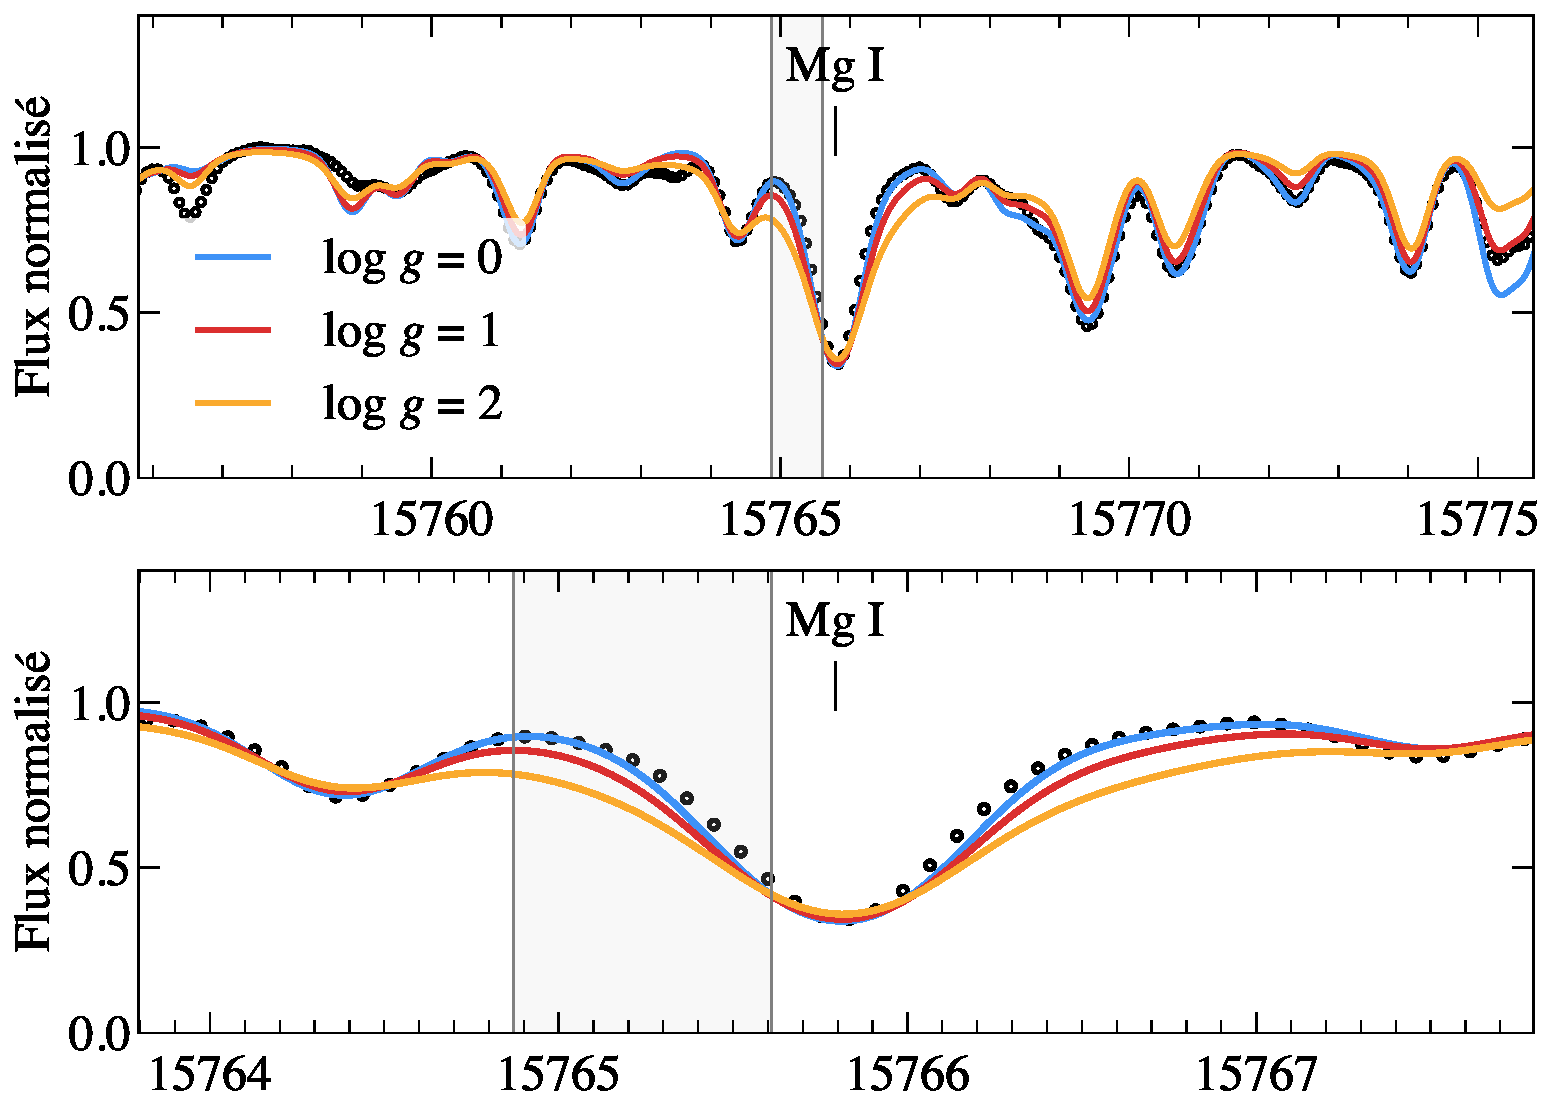
\includegraphics[width=\textwidth]{../output/test4.pdf}  % Insérer le fichier PNG du premier graphique
  \end{subfigure}
  \hfill
  % Deuxième image (graphique 2)
  \begin{subfigure}[b]{0.49\textwidth}  % Augmenter la largeur à 0.48\textwidth
      \centering
      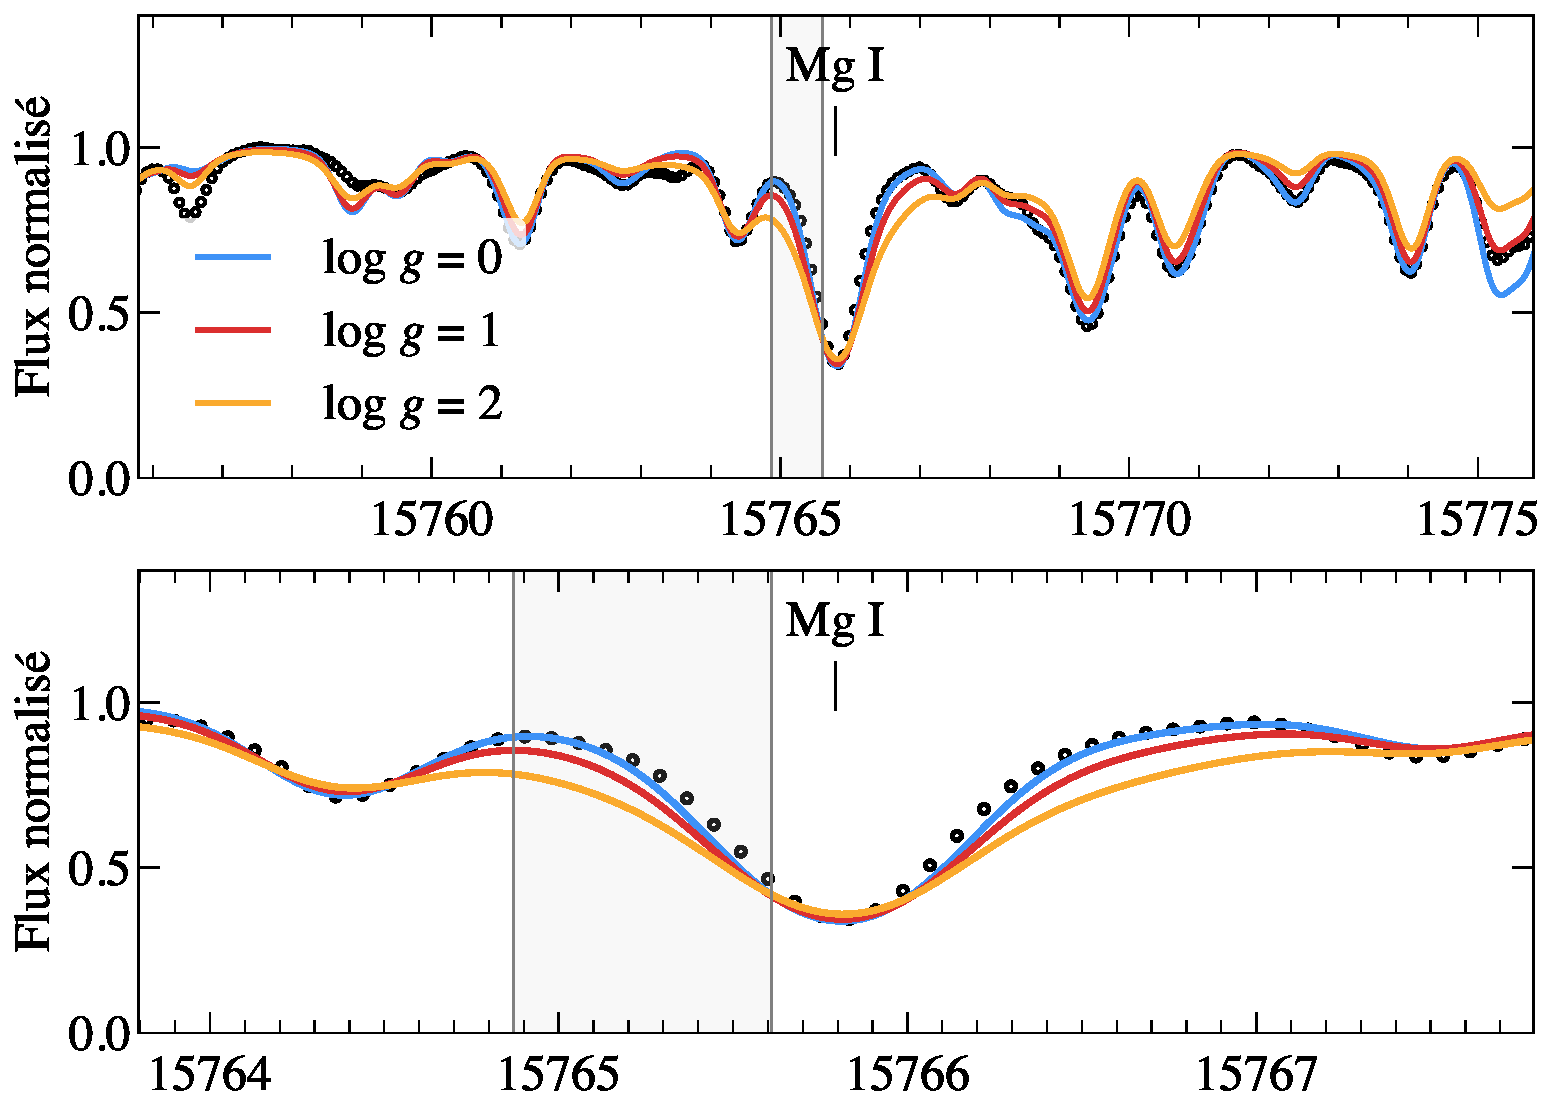
\includegraphics[width=\textwidth]{../output/test4.pdf}  % Insérer le fichier PNG du deuxième graphique
  \end{subfigure}
  
  \vskip 0.3\baselineskip  % Réduire l'espace vertical entre les lignes de graphiques

  % Troisième image (graphique 3)
  \begin{subfigure}[b]{0.49\textwidth}  % Augmenter la largeur à 0.48\textwidth
      \centering
      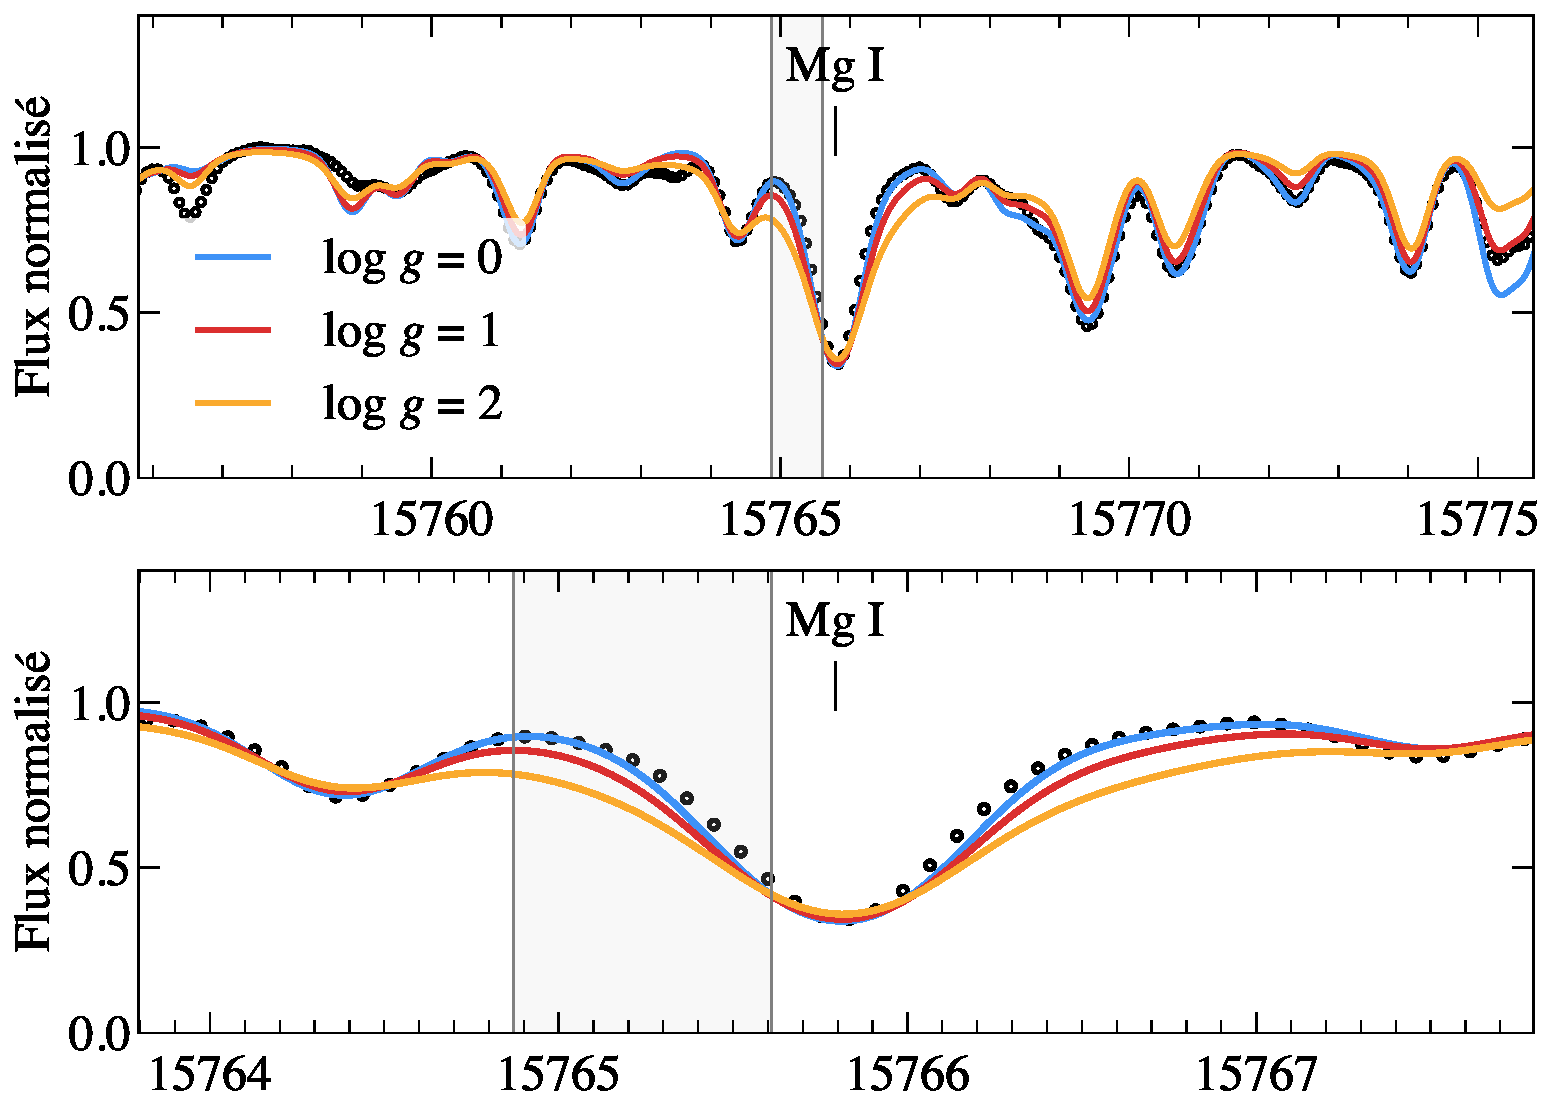
\includegraphics[width=\textwidth]{../output/test4.pdf}  % Insérer le fichier PNG du troisième graphique
  \end{subfigure}
  \hfill
  % Quatrième image (graphique 4)
  \begin{subfigure}[b]{0.49\textwidth}  % Augmenter la largeur à 0.48\textwidth
      \centering
      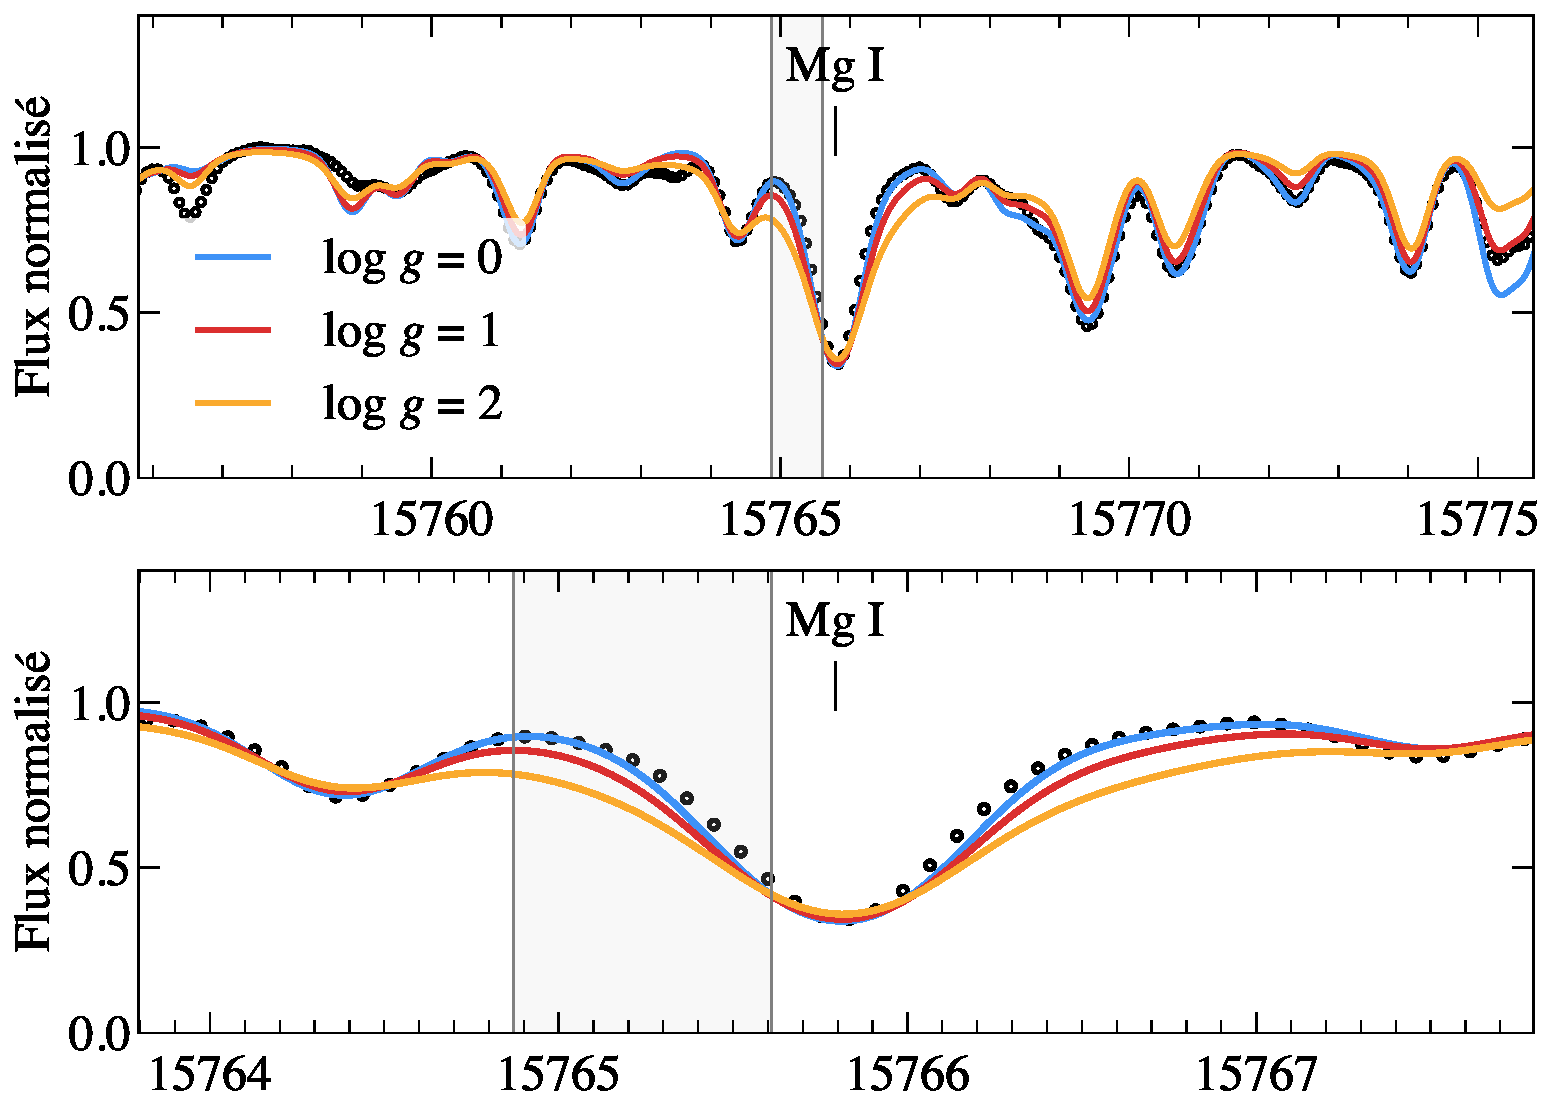
\includegraphics[width=\textwidth]{../output/test4.pdf}  % Insérer le fichier PNG du quatrième graphique
  \end{subfigure}
  \textbf{Notes.}  Variation de la gravité de surface de l'étoile. 
\end{figure}

\section{Métallicité}

log $\varepsilon_{\rm Fe}$ = 7.21
solaire 7.45 
donc [Fe/H] = -0.24 à l'ETL 

\begin{figure}[htbp]
  \begin{center}
  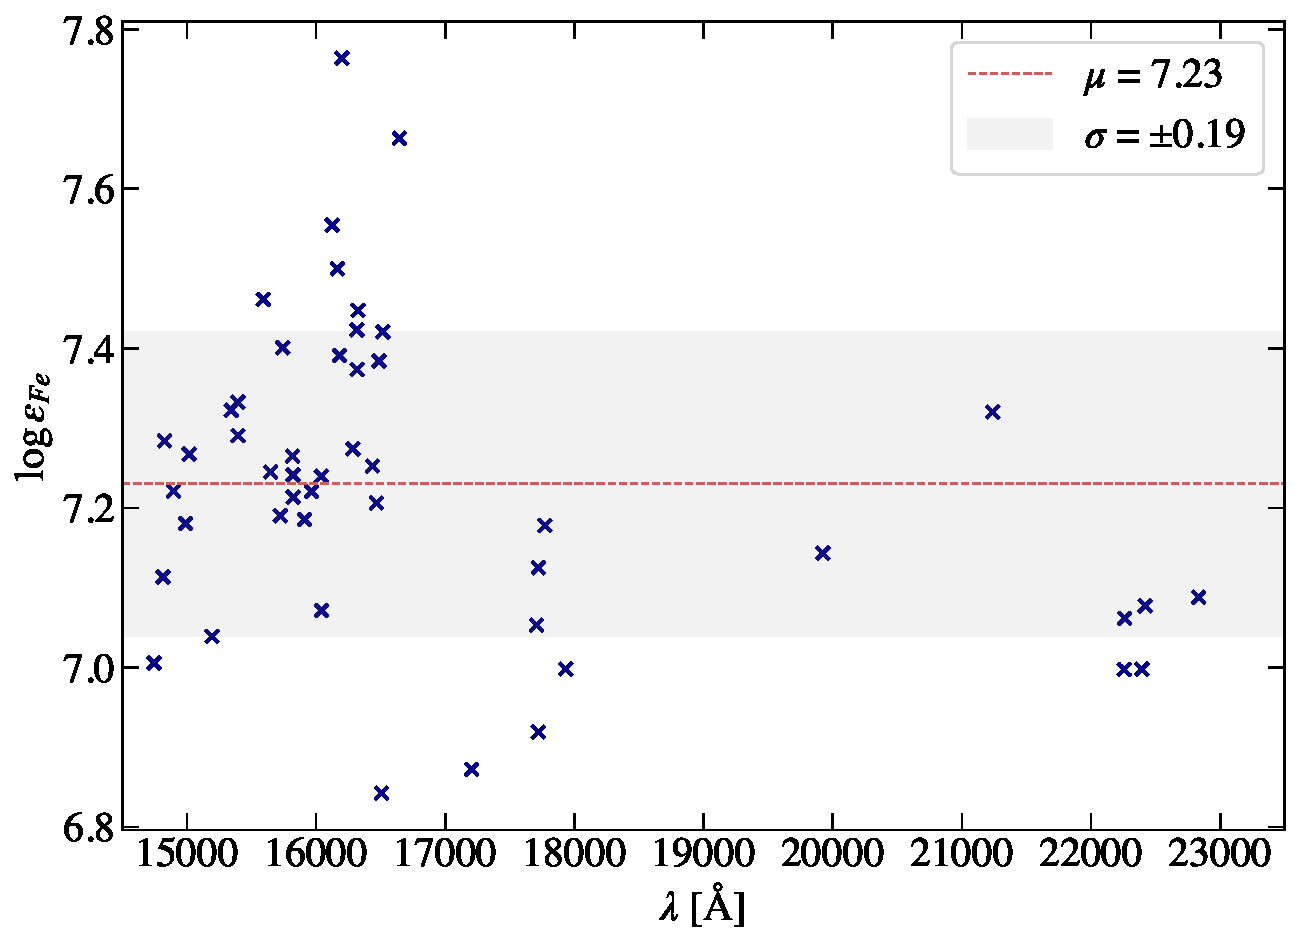
\includegraphics[width=10cm]{images/plot_abu/abu_Fe.pdf}
  \end{center}
  % \caption{Abondance de Fe en fonction de la température effective.}
  \textbf{Notes.}  Abondance de Fe en fonction de la longueur d'onde. Dispersion forte, on regarde en détail les raies de Fe I.
  \label{fig:abu_Fe}
\end{figure}
en 16198.56 frot blendée, on l'élimine.
16645.874 pareil, on l'élimine.

\section{Teff}
pente de quasi 0 donc 4000K bonne Teff à l'ETL 



\section{logg}
on test plusieurs log g avec différents modèles, +1, +2, +0, +3, +4 -> best fit +1 à l'ETL 
sur des raies profondes principalement de Mg et Ca (à tester encore)
checker avec les isochrones et les tracés évolutifs 
l'un suppose l'âge de l'étoile l'autre sa masse



\section{vitesse de micro}
regarder avec eqwuidt la largeur équivalente sinon regarder avec les synthèses et plot python

\section{NLTE}
faire tourner le code poiur les atomes
pas possible de faire de hors etl pour les molécules, même pas pour tous les atomes
\section{abondance d'éléments lourds}
regarder ce que je peux identifier

Ca I, Mg I, Al I, Si I, K I, Ca I, Sc I, Ti II, Ti II, V I, Mn I, Fe I, Co I, Ni I, Cu I,
Y I, Zr I, Ba I, Ce II, Ce III, Er II, Yb II.  

\section{détermination d'abondance}
\begin{table}[h!]
  \vspace{0.3cm}
\begin{center}
	\begin{tabular}{cccccccc}
		\hline
    \hline
        &$\lambda$ & log \textit{gf}&& $\lambda{\rm min}$ & $\lambda{\rm max}$ & $\chi^2$ & log $\varepsilon$ \\
        \hline
        Na I & 19452.98& -0.65 && 19451.82 & 19453.88 & & \\
        & 19505.74& -1.13 && 19504.79 & 19506.51 & & \\
        & 19776.77& -0.39 && 19775.41 & 19777.84 & & \\
        & 19853.09& 0.40 && 19851.97 & 19854.25 & & \\
        & 19862.19& -1.14 && 19861.22 & 19863.30 & & \\
        \hline
      % Na I  & 14767.54 & 14767.03 & 14767.90 & \\
      %   & 14779.69 & 14779.18 & 14780.25 & \\
      %   & 15992.44 & 15991.92 & 15992.86 & \\
      %   & 16373.85 & 16373.32 & 16374.39 & \\
      %   & 16388.86 & 16388.27 & 16389.43 & \\
      %   & 17227.65 & 17227.24 & 17228.07 & \\
      %   & 17227.75 & 17227.24 & 17228.07 & \\
      %   & 18027.85 & 18027.51 & 18028.37 & \\
      %   & 18027.96 & 18027.51 & 18028.37 & \\
      %   & 19796.85 & 19796.46 & 19797.16 & \\
      %   & 21323.78 & 21323.38 & 21324.19 & \\
      %   & 21335.02 & 21334.50 & 21335.56 & \\
      %   & 21452.22 & 21451.42 & 21453.03 & \\
      %   & 21452.38 & 21451.42 & 21453.03 & \\
      %   & 22056.36 & 22055.24 & 22057.55 & \\
      %   & 22083.62 & 22082.62 & 22084.68 & \\
      %   & 23348.37 & 23347.42 & 23349.23 & \\
      %   & 23378.96 & 23377.93 & 23380.27 & \\
      %   & 23379.13 & 23377.93 & 23380.27 & \\
      %   \hline
      % Ce II  & 15277.61 & 15277.30 & 15278.00 & \\
      %   & 15784.79 & 15784.33 & 15785.41 & \\
      %  & 15829.83 & 15829.50 & 15830.43 & \\
      %   & 15958.39 & 15975.91 & 15958.70 & \\
      %   & 15977.12 & 15976.49 & 15977.73 & \\
      %   & 16327.32 & 16326.83 & 16327.84 & \\
      %   & 16376.46 & 16376.00 & 16377.00 & \\
      %  & 16595.23 & 16594.70 & 16595.88 & \\
      %  & 16722.60 & 16721.95 & 16722.92 & \\
      % Ce III  & 15956.79 & 15956.39 & 15957.00 & \\
      %   & 16128.75 & 16128.38 & 16129.00 & \\
      \hline
     Al I & &&& \\


    \end{tabular}
\end{center} 
\textbf{Notes.}  
\label{élément_lourds}
\end{table}
\clearpage

\bibliographystyle{abbrvnat}
\bibliography{bibtex.bib}


\clearpage
\appendix
\section{Table}
\begin{table}[h!]
  %\caption{Listes de molécules et contribution de chacune d'elle dans la bande H et K}
  \vspace{0.3cm}
  \begin{minipage}[t]{.4\linewidth}
  \begin{center}
    \begin{tabular}{ccc}
          \hline
      \hline
      Fe I & $\lambda_{\mathrm{min}}$ & $\lambda_{\mathrm{max}}$ \\
      \hline
          14745.39 & 14745.01 & 14745.93 \\
          14814.73 & 14814.25 & 14815.41 \\
          14826.41 & 14825.87 & 14826.95 \\
          14897.41 & 14896.89 & 14897.82 \\
          14988.78 & 14988.28 & 14989.29 \\
          15017.70 & 15017.25 & 15018.10 \\
          15194.49 & 15194.00 & 15194.93 \\
          15343.79 & 15343.33 & 15344.26 \\
          15394.67 & 15394.21 & 15395.14 \\
          15395.72 & 15395.22 & 15396.31 \\
          15591.49 & 15590.94 & 15591.95 \\
          15648.51 & 15648.03 & 15648.96 \\
          15723.59 & 15723.00 & 15724.01 \\
          15741.92 & 15741.43 & 15742.36 \\
          15818.14 & 15817.57 & 15818.58 \\
          15821.71 & 15821.21 & 15822.14 \\
          15822.82 & 15822.30 & 15823.30 \\
          15911.30 & 15910.82 & 15911.83 \\
          15964.86 & 15964.27 & 15965.43 \\
          16040.65 & 16040.17 & 16041.10 \\
          16042.72 & 16042.18 & 16043.19 \\
          16125.90 & 16125.45 & 16126.45 \\
          16165.03 & 16164.40 & 16165.57 \\
          16180.90 & 16180.44 & 16181.29 \\
          \hline
      \end{tabular}
  \end{center} 
  \end{minipage} 
  \hspace{2.cm}
  \begin{minipage}[t]{.4\linewidth}
  \begin{center}
     \begin{tabular}{ccc}
          \hline
      \hline
      Fe I & $\lambda_{\mathrm{min}}$ & $\lambda_{\mathrm{max}}$ \\
      \hline
      16198.50 & 16197.86 & 16198.95 \\
      16284.77 & 16284.22 & 16285.39 \\
      16316.32 & 16315.75 & 16316.91 \\
      16318.69 & 16318.07 & 16319.23 \\
      16324.45 & 16323.96 & 16325.04 \\
      16436.62 & 16436.19 & 16437.04 \\
      16466.92 & 16466.24 & 16467.55 \\
      16486.67 & 16486.07 & 16487.23 \\
      16506.29 & 16505.74 & 16506.75 \\
      16517.22 & 16516.66 & 16517.67 \\
      16645.87 & 16645.31 & 16646.39 \\
      17204.30 & 17203.74 & 17204.83 \\
      17706.62 & 17705.95 & 17707.11 \\
      17721.09 & 17720.51 & 17721.75 \\
      17721.37 & 17720.51 & 17721.75 \\
      17771.12 & 17770.46 & 17771.70 \\
      17932.60 & 17931.95 & 17933.19 \\
      19923.34 & 19922.62 & 19923.86 \\
      21238.47 & 21237.74 & 21239.13 \\
      22257.11 & 22256.07 & 22257.87 \\
      22260.18 & 22259.25 & 22260.91 \\
      22392.88 & 22392.15 & 22393.39 \\
      22419.98 & 22419.14 & 22420.67 \\
      22832.36 & 22831.40 & 22833.06 \\
          \hline
      \end{tabular}
    \end{center}
  \end{minipage}
  \vspace{0.3cm}
  
  \textbf{Notes.}
  \end{table}

  \begin{table}[h!]
    %\caption{Listes de molécules et contribution de chacune d'elle dans la bande H et K}
    
    \begin{center}
      \vfill
        \begin{tabular}{ccccccc}
        \hline
        \hline
        $^{16}$OH &log \textit{gf}&& $\lambda_{\mathrm{min}}$ & $\lambda_{\mathrm{max}}$ & log $\varepsilon_{O_1}$& $\chi^2_1$\\
        \hline
        14661.14 & -5.99& & 14660.60&14661.59& 8.61&0.015\\
15002.15 & -5.65& & 15001.67&15002.67& 8.62&0.002\\
15003.12 & -5.65& & 15002.67&15003.64& 8.61&0.002\\
15130.92 & -5.57& & 15130.32&15131.53& 8.62&0.002\\
15266.17 & -5.50& & 15265.54&15266.76& 8.61&0.002\\
15278.52 & -5.45& & 15278.03&15279.16& 8.59&0.009\\
15391.20 & -5.51& & 15390.49&15391.93& 8.60&0.001\\
15409.17 & -5.43& & 15408.47&15409.77& 8.60&0.002\\
15428.40 & -5.42& & 15427.96&15429.06& 8.61&0.001\\
15429.69 & -5.15& & 15429.03&15430.13& 8.60&0.001\\
15505.75 & -5.38& & 15504.80&15506.66& 8.59&0.005\\
15568.78 & -5.34& & 15568.17&15569.43& 8.60&0.005\\
15651.90 & -5.20& & 15651.33&15652.41& 8.59&0.003\\
15719.69 & -5.32& & 15719.09&15720.36& 8.60&0.001\\
15755.52 & -5.17& & 15754.86&15756.04& 8.57&0.005\\
15756.53 & -5.17& & 15756.06&15757.10& 8.58&0.003\\
16052.77 & -4.98& & 16052.15&16053.29& 8.58&0.006\\
16247.88 & -5.18& & 16247.50&16248.78& 8.57&0.006\\
16312.92 & -5.08& & 16311.80&16313.42& 8.58&0.003\\
16347.49 & -5.00& & 16347.12&16348.07& 8.62&0.001\\
16368.14 & -4.86& & 16367.51&16368.76& 8.59&0.004\\
16662.20 & -5.07& & 16661.77&16662.85& 8.61&0.001\\
16729.78 & -4.79& & 16729.47&16730.32& 8.58&0.004\\
16904.28 & -4.71& & 16903.62&16904.82& 8.59&0.005\\
17322.25 & -4.63& & 17321.83&17322.84& 8.62&0.003\\
17423.86 & -4.50& & 17423.35&17424.43& 8.59&0.004\\
        \hline
        \end{tabular} \par
        \vspace{1cm}
        \begin{tabular}{ccc}
          \hline
          \hline
          $^{12}$C$^{16}$O & $\lambda_{\mathrm{min}}$ & $\lambda_{\mathrm{max}}$ \\
          \hline
          15780.09 & 15779.54 & 15780.63 \\
          16237.90 & 16237.36 & 16238.29 \\
          16314.39 & 16313.89 & 16314.89 \\
          17026.00 & 17025.60 & 17026.45 \\
          17081.80 & 17081.37 & 17082.30 \\
          17129.35 & 17128.77 & 17129.85 \\
          23073.90 & 23073.11 & 23074.49 \\
          23109.40 & 23108.55 & 23110.21 \\
          \hline
          \end{tabular}
    \end{center} 
    \hspace{2.0cm}
 
    \begin{center}
      \vfill
      \begin{tabular}{ccc}
        \hline
        \hline
        $^{12}$C$^{14}$N & $\lambda_{\mathrm{min}}$ & $\lambda_{\mathrm{max}}$ \\
        \hline
        14744.25 & 14743.77 & 14744.54 \\
        14747.20 & 14746.71 & 14747.72 \\
        14757.56 & 14757.17 & 14757.94 \\
        14759.84 & 14759.41 & 14760.42 \\
        14763.50 & 14762.97 & 14764.06 \\
        14833.25 & 14832.84 & 14833.69 \\
        15192.10 & 15191.68 & 15192.45 \\
        15447.11 & 15446.57 & 15447.58 \\
        16056.95 & 16056.43 & 16057.44 \\
        16167.23 & 16166.88 & 16167.50 \\
        16317.60 & 16317.14 & 16317.92 \\
        16358.15 & 16357.65 & 16358.58 \\
        16590.70 & 16590.39 & 16591.01 \\
        19833.59 & 19833.05 & 19834.02 \\
        19865.84 & 19865.17 & 19866.41 \\
        19906.49 & 19906.00 & 19906.97 \\
        19913.57 & 19912.92 & 19914.17 \\
        22220.20 & 22219.66 & 22220.63 \\
        22400.50 & 22399.90 & 22401.01 \\
        22593.83 & 22593.16 & 22594.40 \\
        22753.90 & 22753.19 & 22754.57 \\
        \hline
        \end{tabular}
      \end{center}
  
    \vspace{0.3cm}
    
    \textbf{Notes.}
    \end{table}



\end{document}  